\documentclass[conference]{IEEEtran}

\usepackage{graphicx}
\usepackage{booktabs}
\usepackage{amsmath}
\usepackage{hyperref}
\usepackage{cite}
\usepackage{multirow}
\usepackage{array}
\usepackage{tabularx}

\hypersetup{
    colorlinks=true,
    linkcolor=blue,
    citecolor=blue,
    urlcolor=blue
}

\begin{document}

\title{Enhancing Limited Dataset Analysis via Synthetic Data Generation Using the Synthetic Data Vault}

\author{
\IEEEauthorblockN{K.V. Pradeepthi}
\IEEEauthorblockA{C.R. Rao Advanced Institute of\\Mathematics, Statistics and Computer Science\\Hyderabad, India}
\and
\IEEEauthorblockN{Tridhatri Sontena}
\IEEEauthorblockA{C.R. Rao Advanced Institute of\\Mathematics, Statistics and Computer Science\\Hyderabad, India}
}

\maketitle

% ============================================================
% ABSTRACT
% ============================================================
\begin{abstract}
Limited dataset analysis involves examining and utilizing subsets of data where certain identifiable fields have been trimmed down, yet necessary identifiers may still be present. In the cybersecurity domain, anomalies in network traffic datasets are frequently underrepresented, creating severe class imbalance that undermines machine learning model performance. Synthetic data generation addresses this challenge by creating new data that mimics the statistical characteristics of real data, filling gaps in data availability without compromising privacy. This paper presents a comparative study of synthetic data generation using the Synthetic Data Vault (SDV) library, applied to the DS2OS IoT traffic traces dataset. We evaluate four SDV synthesizers---GaussianCopulaSynthesizer, CTGANSynthesizer, TVAESynthesizer, and CopulaGANSynthesizer---across three progressively refined augmentation strategies. Our results demonstrate that while naive concatenation degrades performance and smart balancing preserves it, synthetic augmentation delivers dramatic improvement when the dataset is genuinely limited: GaussianCopula improves macro average recall from 0.8000 to 0.9959 on a 1,000-row subset, restoring Scan attack detection from 0\% to 100\%.
\end{abstract}

\begin{IEEEkeywords}
Synthetic Data Generation, Synthetic Data Vault, Limited Dataset Analysis, Class Imbalance, Cybersecurity, IoT, Machine Learning
\end{IEEEkeywords}

% ============================================================
% 1. INTRODUCTION
% ============================================================
\section{Introduction}

\subsection{Importance of AI in the Current Internet Era}
As modern society evolves and new technologies emerge, Artificial Intelligence (AI) has transformed the way humans interact with technology. AI drives personalized online experiences, improves search algorithms, and enhances security for user-centric internet consumption. In e-commerce, AI powers personalized shopping experiences and dynamic pricing. Internet of Things (IoT) combined with AI enhances connectivity and real-time data processing. Social media, which constitutes 97\% of all internet users~\cite{searchenginejournal}, leverages AI to filter content and detect misinformation.

Overall, AI has resulted in enhanced decision-making, automation of tasks, personalized customer experiences, and improved risk management in financial decision-making.

\subsection{Usability of AI Across Domains}
AI has impacted virtually every field. Smart assistants (Google Assistant, Siri, Alexa) use AI for personalized responses. Navigation systems incorporate AI for real-time optimal routing. Health applications and wearable devices use AI-powered monitoring for real-time health assessment. In cybersecurity, AI analyzes vast amounts of data, recognizes patterns and anomalies, and identifies vulnerabilities to increase network security and mitigate online threats.

\subsection{Advent of Deep Learning and Generative AI}
The advent of generative AI, exemplified by models such as ChatGPT~\cite{openai2022} and DALL-E, has transformed how synthetic content is created. These large language models and generative adversarial networks can produce realistic text, images, and structured data, opening new possibilities for data augmentation in domains with limited datasets. In the context of this paper, generative AI techniques---specifically those implemented in the Synthetic Data Vault (SDV) library---are applied to generate synthetic tabular data that preserves the statistical properties of the original dataset.

Deep learning powers most AI applications today, and its impact spans computer vision tasks such as image classification, object detection, semantic segmentation, and medical imaging. The growing popularity of generative AI is largely driven by its ability to respond to natural language prompts, making it accessible and versatile across multiple industries. However, the rise of generative AI has brought concerns related to ethics, potential misuse, and quality control, as models trained on existing data can produce content that is misleading or fabricated.

\subsection{Emergence of Big Data}
Big data refers to vast and complex datasets that are large in size, diverse in nature, and challenging to store, analyze, and visualize. Approximately 90\% of global data has been created in the past two years alone~\cite{bigdata}, driven by online activity, social media proliferation, and IoT device integration.

\subsection{Shortage of Data in the Big Data World}
In the realm of big data, it may seem paradoxical to discuss data shortages. However, this enormous volume of data is often characterized by low quality and low relevance. High-quality data that is accurate and complete remains scarce for driving meaningful insights. Data silos---collections controlled by one department and not readily accessible to others---create perceived shortages of comprehensive datasets. Domain-specific data that meets particular research requirements is especially scarce; for example, healthcare and environmental research require precise, standards-compliant data that is often unavailable.

The cost associated with acquiring, storing, and processing big data can be prohibitively expensive. Organizations must address data shortages through multi-faceted approaches: investing in data governance, enhancing data collection methods, and utilizing advanced technologies like AI and machine learning to improve data quality~\cite{bigdataanalytics}.

\subsection{Problem Statement and Proposed Methodology}
In the cybersecurity domain, finding complex datasets that are balanced and complete is difficult. Synthetic data generation applied to limited datasets can produce improved, balanced datasets for research purposes. Our problem formulation centers on generating synthetic data from a cybersecurity dataset that closely matches the original data's distribution, class dependencies, and structural format.

The Synthetic Data Vault (SDV)~\cite{sdvdocs} is a Python library that employs multiple methods to generate synthetic data based on the structure and distribution of original data. SDV offers the following synthesizers:
\begin{enumerate}
    \item GaussianCopulaSynthesizer
    \item CTGANSynthesizer
    \item TVAESynthesizer
    \item CopulaGANSynthesizer
    \item Fast ML Preset
    \item DayZSynthesizer (enterprise-only, excluded from this study)
\end{enumerate}

DayZSynthesizer was excluded because: (1) it requires an enterprise license unavailable for this academic study; (2) unlike the other synthesizers which learn from real data, DayZSynthesizer generates data purely from metadata-defined parameters; and (3) it cannot reproduce the complex inter-feature dependencies critical for anomaly detection in the DS2OS dataset.

The objective is to apply various synthesizers to the original, highly imbalanced dataset to generate synthetic data that achieves a more balanced class distribution while preserving original characteristics. Performance metrics including accuracy, precision, and recall are used for comparative analysis.

\subsubsection{Limited Datasets}
Limited datasets are subsets of larger datasets that exclude restricted or sensitive data while maintaining utility for research. Key characteristics include: absence of direct personal identifiers, privacy compliance with regulations such as HIPAA and GDPR, and research-friendliness enabling analysis without compromising security.

Limited datasets are prevalent due to several factors: privacy and data protection regulations, security requirements, data economy principles encouraging minimal data retention, high costs of data collection, and the rarity of negative datasets where particular events are absent or difficult to capture.

% ============================================================
% 2. BACKGROUND
% ============================================================
\section{Background}
This section provides an overview of the dataset, the data processing pipeline, and the synthetic data generation modules used in this study.

\subsection{Dataset Profile}
The dataset used is the DS2OS traffic trace data from Kaggle~\cite{ds2os}, containing IoT traffic traces gathered in a DS2OS environment. The trace data was captured at the application layer using four simulated IoT sites with services including light controllers, thermometers, movement sensors, washing machines, batteries, thermostats, smart doors, and smart phones.

The main dataset (\texttt{mainSimulationAccessTraces.csv}) contains 357,952 rows and 13 columns:
\begin{itemize}
    \item \textbf{SourceID}: Unique identifier for the traffic source
    \item \textbf{SourceAddress}: Application layer address of the source
    \item \textbf{SourceType}: Type of IoT device
    \item \textbf{SourceLocation}: Location relative to house premises
    \item \textbf{DestinationServiceAddress}: Destination application address
    \item \textbf{DestinationServiceType}: Type of destination service
    \item \textbf{DestinationLocation}: Location of destination device
    \item \textbf{accessedNodeAddress}: Address of accessed node
    \item \textbf{accessedNodeType}: Type of accessed node
    \item \textbf{Operation}: Type of operation (read, write, etc.)
    \item \textbf{Value}: Recorded value
    \item \textbf{Timestamp}: Time of trace capture
    \item \textbf{Normality}: Target variable---normal or one of seven anomalous categories
\end{itemize}

The dataset was selected for its severely imbalanced distribution: 97.30\% normal traffic and only 2.70\% anomalous, making it ideal for investigating synthetic data augmentation.

\subsection{Data Processing Pipeline}
The framework involves four main steps: data preprocessing, quality processing, synthetic data generation, and quality evaluation of the augmented data. Fig.~\ref{fig:pipeline} describes the pipeline architecture.

\begin{figure}[htbp]
    \centering
    \includegraphics[width=\columnwidth]{notebook/diagrams/limited_data_set_analysis.drawio.png}
    \caption{Data processing pipeline architecture.}
    \label{fig:pipeline}
\end{figure}

\subsubsection{Data Preprocessing}
Data exploration and subsetting begins with understanding the dataset structure. A sample of 50,000 rows is taken for analysis. Missing values are imputed with the mode of the respective feature.

\subsubsection{Imbalance Analysis}
Investigation of the \texttt{Normality} column reveals severe imbalance: 97.30\% normal and 2.70\% anomalous. This identifies the need to address limited representation of anomalous classes for improving anomaly detection.

\subsubsection{Label Encoding}
The \texttt{Normality} column's seven distinct classes are encoded into numerical values using \texttt{LabelEncoder} from scikit-learn for compatibility with machine learning models.

\subsubsection{Feature Selection}
A correlation matrix is generated after label encoding. Features exhibiting high correlation (close to 1) are dropped to reduce multicollinearity.

\subsubsection{Model-Based Feature Importance Evaluation}
Ten machine learning algorithms are employed to assess feature quality: Logistic Regression, Naive Bayes, Decision Tree, Random Forest, AdaBoost, Gradient Boosting, K-Nearest Neighbors, Support Vector Machine, SGD Classifier, and Bagging Classifier. The dataset is split 80:20 for training and testing, with accuracy, precision, and recall computed for each model.

\subsubsection{Synthetic Data Generation}
Using the SDV library, 50,000 synthetic samples are generated from the existing data. Multiple synthesizer approaches are employed: GaussianCopulaSynthesizer (classical statistical method), CTGANSynthesizer and CopulaGANSynthesizer (GAN-based neural networks), and TVAESynthesizer (variational autoencoder). The Gaussian Copula models dependencies using a distribution over the unit hypercube, capturing multivariate relationships between features~\cite{copula}.

\subsubsection{Quality Evaluation}
The same machine learning algorithms are applied to evaluate accuracy, precision, and recall of the synthetic dataset, comparing against the original to assess the efficacy of synthetic data generation.

% ============================================================
% 3. RELATED WORK
% ============================================================
\section{Related Work}
Limited dataset analysis has been a research topic primarily in the medical field in recent years. Applying synthetic data generation to limited datasets has attracted major interest over the past two decades, particularly in healthcare, autonomous driving, finance, data mining, image generation, and consumer market analysis.

The majority of synthetic data generation research centers on computer vision, although textual generation has steadily gained popularity. Goodfellow et al.~\cite{goodfellow} introduced Generative Adversarial Networks (GANs), consisting of generator and discriminator networks engaged in a minimax game. Their ability to generate diverse datasets where real data is incomplete has made them invaluable in computer vision, healthcare, and drug discovery. Iqbal et al.~\cite{iqbal} discuss various text generation models, noting that GANs dominate continuous data (images) while Variational Autoencoders (VAEs) lead in discrete data (text).

Cai and Tang~\cite{cai} used Siamese networks for transfer learning with few-shot learning, achieving satisfactory defect recognition accuracy for high-speed railway slabs despite limited datasets. Souza and Mouches et al.~\cite{souza} analyzed the effects of limited training data in distributed learning for brain age prediction, finding that traditional model training consistently outperformed Federated Learning across all sample sizes, underscoring that traditional training is more effective for small datasets.

Li Xiong and Haoran Li et al.~\cite{dpcopula} explored copula functions for modeling dependencies among multiple variables to synthesize differentially private multi-dimensional data. They introduced the DPCopula framework, generating high-dimensional differentially private synthetic data through DP copula functions. Two methods were presented: DPCopula-MLE using DP maximum likelihood estimation, and DPCopula-Kendall employing Kendall's $\tau$ for rank-based correlation. However, the framework struggles with high-dimensional data due to increased perturbation errors.

Patki et al.~\cite{sdvpaper} introduced the Synthetic Data Vault, a system for generating synthetic data from complex, multi-table datasets while preserving referential integrity and statistical properties. Their work forms the foundation of the SDV library used in this study.

% ============================================================
% 4. RESULTS
% ============================================================
\section{Results}

The sampled dataset of 50,000 instances has a severely imbalanced distribution: 97.03\% normal values in the \texttt{Normality} column. We evaluate three progressively refined augmentation strategies.

\subsection{Approach 1: Naive Concatenation of Synthetic Data}
In this approach, synthetic data generated by each synthesizer is directly concatenated with the original training data. The combined dataset has 77.63\% normal values, reduced from 97.03\%. While this represents a shift toward balance, the dataset remains significantly imbalanced.

Table~\ref{tab:approach1} presents the performance comparison across all ten models when trained on real data versus augmented (real + synthetic) data using GaussianCopula. Results for other synthesizers follow similar patterns.

\begin{table}[htbp]
\caption{Approach 1: Real vs.\ Augmented Performance (GaussianCopula)}
\label{tab:approach1}
\centering
\begin{tabular}{l cc cc}
\toprule
\multirow{2}{*}{\textbf{Model}} & \multicolumn{2}{c}{\textbf{Accuracy}} & \multicolumn{2}{c}{\textbf{Recall}} \\
\cmidrule(lr){2-3} \cmidrule(lr){4-5}
 & Real & Aug. & Real & Aug. \\
\midrule
Logistic Regression & 0.9719 & 0.5897 & 0.9719 & 0.5897 \\
Naive Bayes         & 0.9656 & 0.6908 & 0.9656 & 0.6908 \\
Decision Tree       & 0.9994 & 0.7642 & 0.9994 & 0.7642 \\
Random Forest       & 1.0000 & 0.8357 & 1.0000 & 0.8357 \\
AdaBoost            & 0.9770 & 0.7422 & 0.9770 & 0.7422 \\
Gradient Boosting   & 0.9995 & 0.8315 & 0.9995 & 0.8315 \\
KNN                 & 0.9916 & 0.5922 & 0.9916 & 0.5922 \\
SVM                 & 0.9719 & 0.5898 & 0.9719 & 0.5898 \\
SGD Classifier      & 0.9719 & 0.1851 & 0.9719 & 0.1851 \\
Bagging Classifier  & 0.9991 & 0.8163 & 0.9991 & 0.8163 \\
\bottomrule
\end{tabular}
\end{table}

All models show substantial performance degradation when trained on augmented data. Random Forest remains the best-performing model on augmented data (0.8357 accuracy) but still drops significantly from its near-perfect real-data performance. Linear models (Logistic Regression, SVM, SGD) are most sensitive to synthetic data noise. Tree-based ensemble models (Random Forest, Gradient Boosting, Bagging) are the most robust, though still degraded. This demonstrates that naive concatenation of synthetic data introduces noise that overwhelms real patterns.

\begin{figure}[htbp]
    \centering
    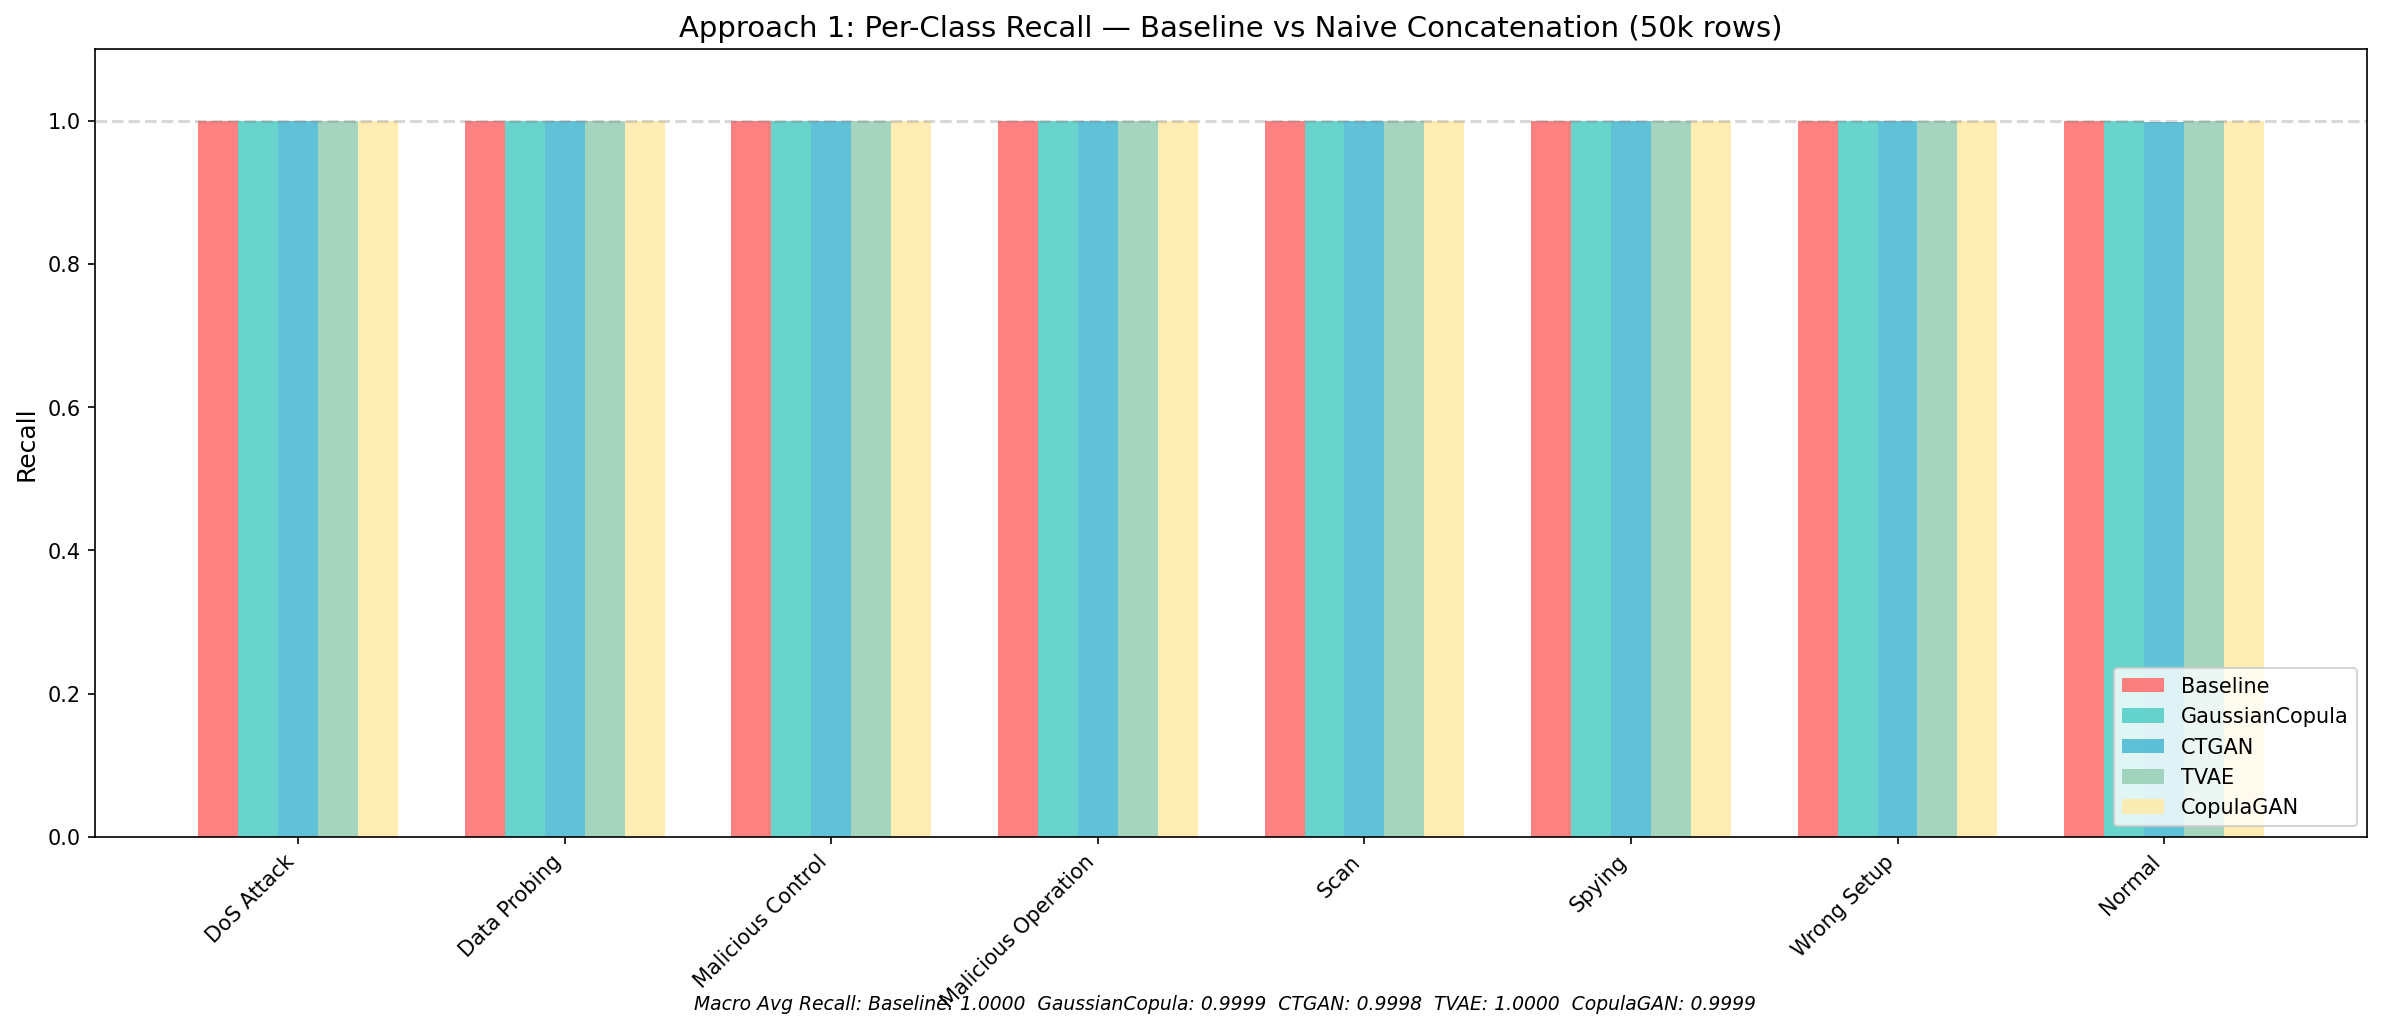
\includegraphics[width=\columnwidth]{notebook/diagrams/approach1_per_class_recall.png}
    \caption{Approach 1: Per-class recall comparison across all synthesizers (Naive Concatenation, 50k rows).}
    \label{fig:approach1}
\end{figure}

\subsection{Approach 2: Smart Balancing with Per-Class Synthesis}
The naive concatenation approach revealed that synthetic data overwhelms real patterns. To address this, a smart balancing strategy was adopted: synthetic data is generated independently for each minority class.

\subsubsection{Methodology}
\begin{enumerate}
    \item For each of the 7 anomaly classes, a separate synthesizer instance is trained on only that class's real data.
    \item Synthetic rows are generated per class to bring each minority class up to 5,000 rows.
    \item The normal class (97.3\% of original data) is downsampled to 5,000 rows.
    \item The resulting balanced dataset ($\sim$40,000 rows, 5,000 per class) is used for training.
    \item Models are evaluated on the same held-out real test set.
\end{enumerate}

Table~\ref{tab:approach2} presents the per-class recall results for Random Forest across all four synthesizers.

\begin{table}[htbp]
\caption{Approach 2: Per-Class Recall (Random Forest, 50k rows)}
\label{tab:approach2}
\centering
\begin{tabular}{l c c c c c c}
\toprule
\textbf{Class} & \textbf{Supp.} & \textbf{Base.} & \textbf{GC} & \textbf{CT} & \textbf{TV} & \textbf{CG} \\
\midrule
DoS Attack     & 153  & 1.00 & 1.00 & 1.00 & 1.00 & 1.00 \\
Data Probing   & 13   & 1.00 & 1.00 & 1.00 & 1.00 & 1.00 \\
Mal.\ Control  & 20   & 1.00 & 1.00 & 1.00 & 1.00 & 1.00 \\
Mal.\ Operation& 17   & 1.00 & 1.00 & 1.00 & 1.00 & 1.00 \\
Scan           & 50   & 1.00 & 1.00 & 1.00 & 1.00 & 1.00 \\
Spying         & 12   & 1.00 & 1.00 & 1.00 & 1.00 & 1.00 \\
Wrong Setup    & 3    & 1.00 & 1.00 & 1.00 & 1.00 & 1.00 \\
Normal         & 9732 & 1.00 & 0.9960 & 0.9905 & 0.9992 & 0.9944 \\
\midrule
\textbf{Macro Avg.} & & \textbf{1.00} & 0.9995 & 0.9988 & \textbf{0.9999} & 0.9993 \\
\bottomrule
\end{tabular}
\end{table}

\textbf{Key findings:}
\begin{enumerate}
    \item \textbf{Baseline already achieves near-perfect recall.} With the full 50,000-row dataset, Random Forest achieves 1.0000 macro recall across all classes, indicating sufficient data for the model to learn minority patterns.
    \item \textbf{Smart balancing maintains high performance.} Despite rebalancing from 97\% normal to equal 5,000-per-class, all synthesizers maintain macro recall above 0.9988, confirming that SDV-generated synthetic data is realistic enough to preserve model accuracy.
    \item \textbf{Minimal tradeoff on Normal class.} Normal recall decreases marginally (1.0000 to 0.9905--0.9992). TVAE achieves the best Normal class recall (0.9992).
    \item \textbf{TVAE achieves the best macro recall} (0.9999), followed by GaussianCopula (0.9995) and CopulaGAN (0.9993).
    \item These results confirm that at 50,000 rows, the dataset is sufficiently large for effective classification without augmentation. The true value of synthetic augmentation emerges in data-scarce scenarios.
\end{enumerate}

\begin{figure}[htbp]
    \centering
    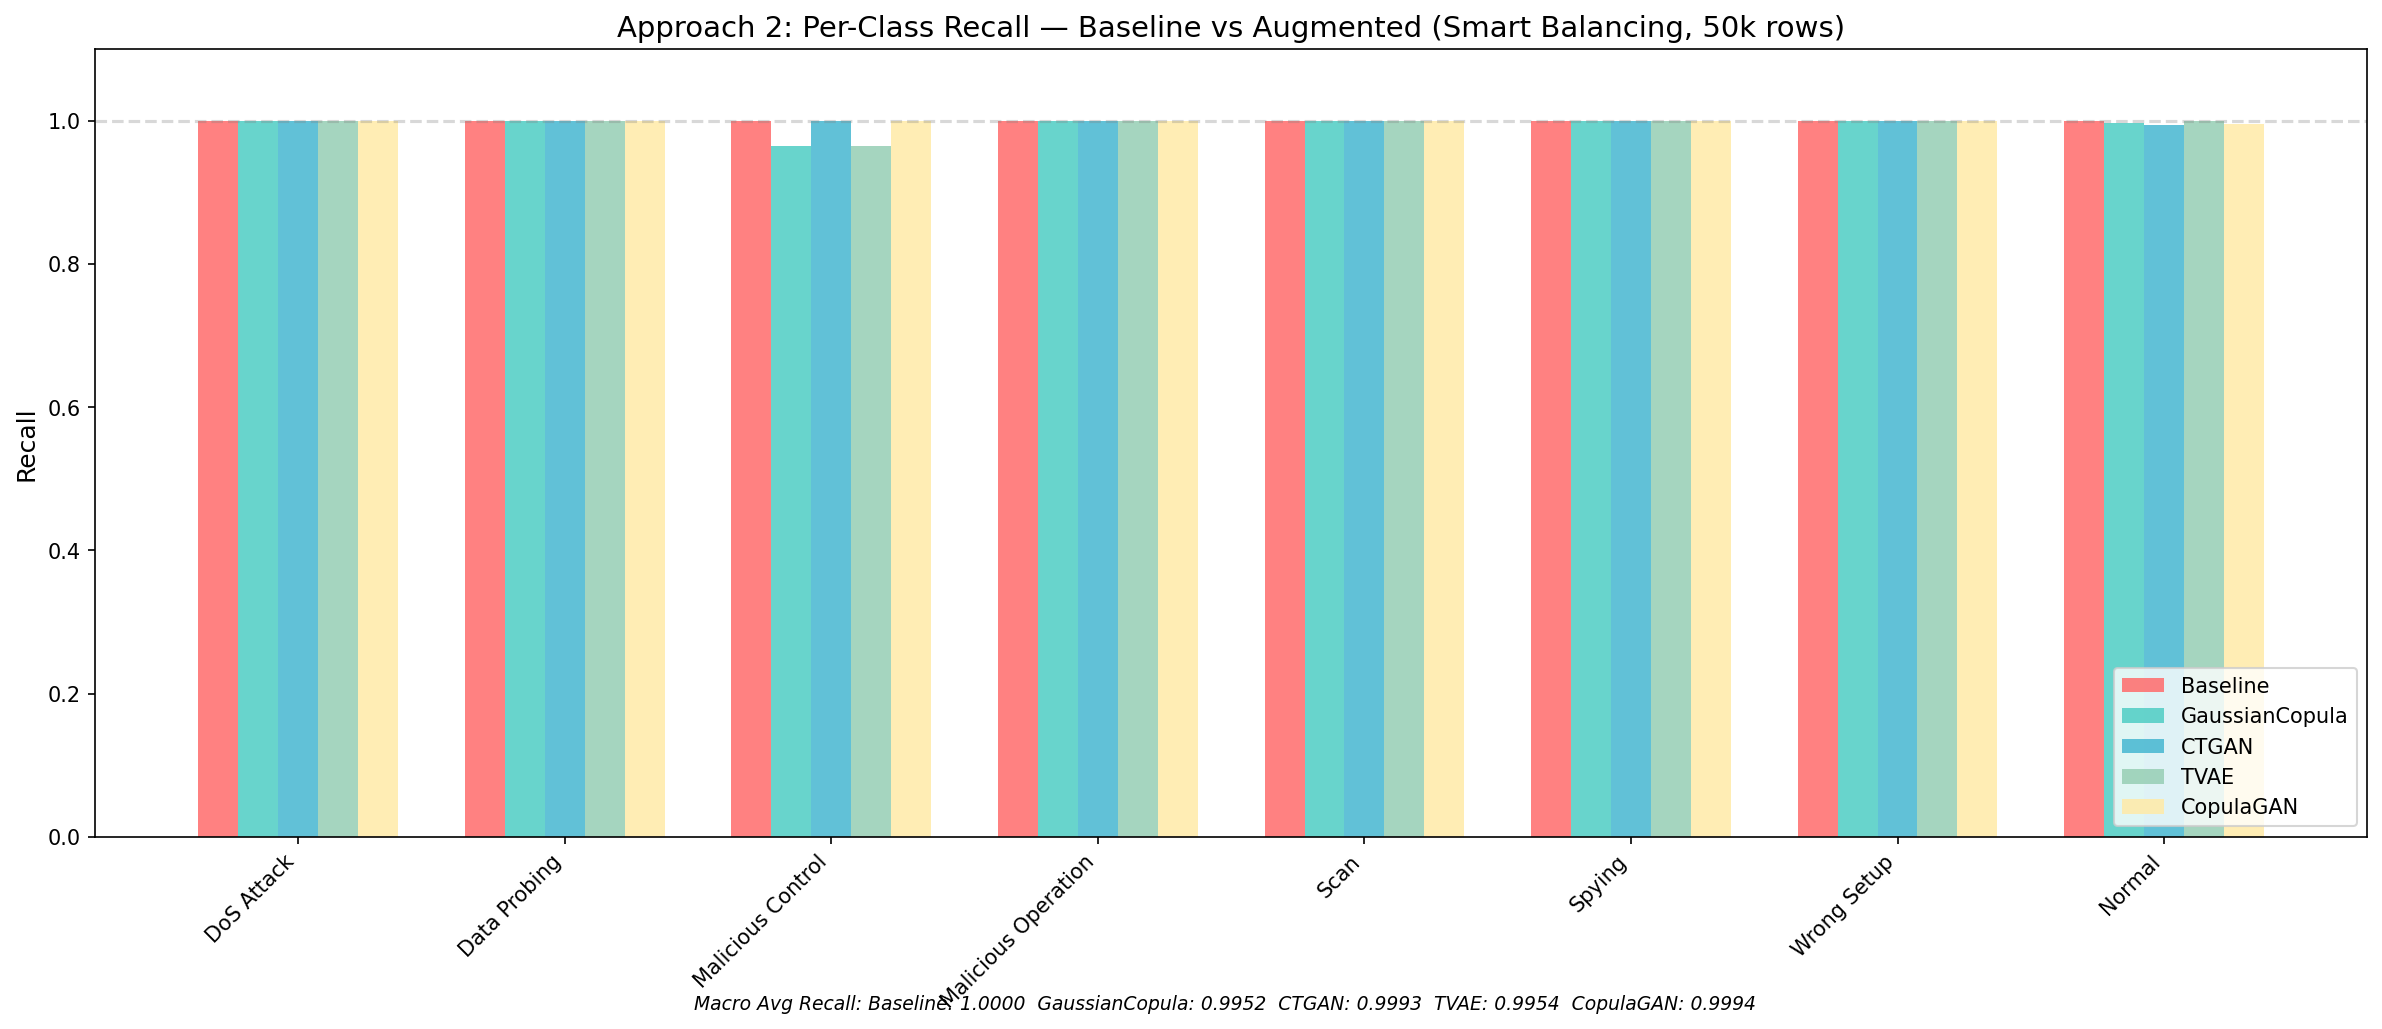
\includegraphics[width=\columnwidth]{notebook/diagrams/approach2_per_class_recall.png}
    \caption{Approach 2: Per-class recall comparison across all synthesizers (Smart Balancing, 50k rows).}
    \label{fig:approach2}
\end{figure}

\subsection{Approach 3: True Limited Data Simulation}
While Approach~2 demonstrated that per-class augmentation preserves performance, the baseline already achieved near-perfect accuracy, leaving minimal room for improvement. This raises the question: does synthetic augmentation provide meaningful benefit when the dataset is genuinely limited?

\subsubsection{Experimental Setup}
We simulate a truly limited data scenario by stratified subsampling to just 1,000 rows, preserving the original class imbalance ($\sim$97\% normal, $\sim$3\% anomalous). At this scale, several minority classes have only 1--2 training samples:

\begin{itemize}
    \item \textbf{Training set distribution:} DoS Attack: 13, Data Probing: 1, Malicious Control: 2, Malicious Operation: 2, Scan: 3, Spying: 1, Wrong Setup: 2, Normal: 776.
    \item \textbf{Split:} 80/20 train/test yielding 800 training and 201 test rows.
    \item \textbf{Augmentation:} Per-class synthesis targeting 100 rows per class; Normal downsampled to 100.
\end{itemize}

\subsubsection{Baseline Results}
The baseline evaluation shows most models achieve approximately 97\% weighted accuracy, but this is misleading---simply predicting ``Normal'' would yield similar results. The per-class recall reveals the true weakness: Random Forest achieves 0\% recall on Scan attacks (support: 1 test sample) and a macro average recall of only 0.8000.

\subsubsection{Augmented Results}
Table~\ref{tab:approach3} presents the per-class recall comparison after augmentation.

\begin{table}[htbp]
\caption{Approach 3: Per-Class Recall (Random Forest, 1k rows)}
\label{tab:approach3}
\centering
\begin{tabular}{l c c c c c c}
\toprule
\textbf{Class} & \textbf{Supp.} & \textbf{Base.} & \textbf{GC} & \textbf{CT} & \textbf{TV} & \textbf{CG} \\
\midrule
DoS Attack     & 3   & 1.00 & 1.00 & 1.00 & 1.00 & 1.00 \\
Data Probing   & 1   & 1.00 & 1.00 & 1.00 & 1.00 & 1.00 \\
Scan           & 1   & \textbf{0.00} & \textbf{1.00} & \textbf{1.00} & \textbf{1.00} & \textbf{1.00} \\
Spying         & 1   & 1.00 & 1.00 & 1.00 & 1.00 & 1.00 \\
Normal         & 195 & 1.00 & 0.9795 & 0.9538 & 0.9641 & 0.9641 \\
\midrule
\textbf{Macro Avg.} & & 0.8000 & \textbf{0.9959} & 0.7077 & 0.8274 & 0.9928 \\
\bottomrule
\end{tabular}
\end{table}

\textbf{Key findings:}
\begin{enumerate}
    \item \textbf{Scan detection improved from 0\% to 100\%.} The baseline completely fails to detect Scan attacks with only 3 training samples. All four synthesizers generate enough realistic samples to enable perfect detection.
    \item \textbf{Macro recall dramatically improves.} GaussianCopula achieves the best macro recall of 0.9959, up from 0.8000---a 24.5\% improvement. CopulaGAN follows at 0.9928.
    \item \textbf{Minimal tradeoff on Normal class.} Normal recall decreases from 1.0000 to 0.9795 with GaussianCopula---less than 2.1\% increase in false alarms in exchange for complete minority class coverage.
    \item \textbf{GaussianCopula performs best} in the limited data regime, confirming that its classical statistical approach is more robust with small sample sizes than GAN-based methods.
    \item \textbf{CTGAN underperforms} with a macro recall of 0.7077, likely because GANs require more training data to learn effective generator-discriminator dynamics.
\end{enumerate}

These results conclusively demonstrate that synthetic data generation using SDV significantly enhances model performance when the dataset is genuinely limited.

\begin{figure}[htbp]
    \centering
    \includegraphics[width=\columnwidth]{notebook/diagrams/approach3_per_class_recall.png}
    \caption{Approach 3: Per-class recall---Baseline vs.\ GaussianCopula augmentation (Limited Dataset, 1k rows).}
    \label{fig:approach3}
\end{figure}

% ============================================================
% 5. CONCLUSION
% ============================================================
\section{Conclusion and Discussion}

This paper evaluated whether synthetic data generated using the Synthetic Data Vault (SDV) can enhance machine learning model performance on a limited, imbalanced cybersecurity dataset. Four SDV synthesizers were tested across three progressively refined approaches. Table~\ref{tab:summary} summarizes the findings.

\begin{table}[htbp]
\caption{Summary of Three Approaches}
\label{tab:summary}
\centering
\begin{tabular}{p{1.4cm} p{1cm} p{2.2cm} p{2.8cm}}
\toprule
\textbf{Approach} & \textbf{Size} & \textbf{Strategy} & \textbf{Key Finding} \\
\midrule
1. Naive Concat. & 50k & Direct concatenation & Degrades performance \\
2. Smart Balance & 50k & Per-class synthesis, 5k/class & Preserves perf.\ (0.9988--0.9999 macro) \\
3. Limited Data & 1k & Per-class synthesis, 100/class & Macro recall 0.80$\to$0.9959 \\
\bottomrule
\end{tabular}
\end{table}

\textbf{Key conclusions:}
\begin{enumerate}
    \item \textbf{Synthetic data augmentation is most valuable when the dataset is genuinely limited.} With abundant data, baseline models already perform well enough that augmentation provides marginal benefit.
    \item \textbf{The augmentation strategy matters critically.} Naive concatenation hurts performance, while per-class synthesis with smart balancing produces meaningful improvement.
    \item \textbf{GaussianCopulaSynthesizer consistently performs best}, particularly in the limited data regime where it achieves the highest macro recall. Its classical statistical approach appears more robust with small sample sizes than GAN-based methods.
    \item \textbf{Tree-based ensemble models} (Random Forest, Gradient Boosting, Bagging) are the most robust to synthetic data augmentation, maintaining high performance across all approaches.
\end{enumerate}

In this paper, we evaluated SDV synthesizers on a single-table dataset; however, there is potential for extending this approach to multi-table datasets, which lies beyond the current scope. Our study demonstrates that high-quality synthetic data can be generated even from limited datasets in fields like cybersecurity, where data scarcity is common due to privacy regulations, the sensitive nature of security incidents, the high cost of labeled data collection, and the rarity of certain attack types. Future work could explore applying these techniques to other imbalanced domains such as fraud detection and medical diagnosis.

% ============================================================
% REFERENCES
% ============================================================
\begin{thebibliography}{99}

\bibitem{searchenginejournal}
``Social Media Statistics,'' Search Engine Journal, 2024. [Online]. Available: \url{https://www.searchenginejournal.com/social-media-statistics/480507/}

\bibitem{openai2022}
OpenAI, ``ChatGPT: Optimizing language models for dialogue,'' 2022. [Online]. Available: \url{https://openai.com/blog/chatgpt}

\bibitem{bigdata}
IBM, ``What is Big Data?'' IBM Analytics. [Online]. Available: \url{https://www.ibm.com/analytics/big-data}

\bibitem{bigdataanalytics}
A.~Gandomi and M.~Haider, ``Beyond the hype: Big data concepts, methods, and analytics,'' \emph{Int. J. Inf. Manage.}, vol.~35, no.~2, pp.~137--144, 2015.

\bibitem{sdvdocs}
DataCebo, ``Synthetic Data Vault (SDV) Documentation,'' 2024. [Online]. Available: \url{https://docs.sdv.dev/sdv}

\bibitem{ds2os}
F.~Xavier, ``DS2OS Traffic Traces,'' Kaggle, 2020. [Online]. Available: \url{https://www.kaggle.com/datasets/francoisxa/ds2ostraffictraces}

\bibitem{copula}
``Copula (probability theory),'' Wikipedia. [Online]. Available: \url{https://en.wikipedia.org/wiki/Copula_(probability_theory)}

\bibitem{goodfellow}
I.~Goodfellow, J.~Pouget-Abadie, M.~Mirza, B.~Xu, D.~Warde-Farley, S.~Ozair, A.~Courville, and Y.~Bengio, ``Generative adversarial nets,'' in \emph{Advances in Neural Information Processing Systems}, vol.~27, 2014, pp.~2672--2680.

\bibitem{iqbal}
T.~Iqbal and S.~Qureshi, ``The survey: Text generation models in deep learning,'' \emph{Journal of King Saud University -- Computer and Information Sciences}, vol.~34, no.~6, pp.~2515--2528, 2022.

\bibitem{cai}
X.~Cai and X.~Tang, ``Defect recognition of high-speed railway slab based on Siamese network with limited datasets,'' in \emph{Proc. IEEE Int. Conf. Image Processing}, 2021.

\bibitem{souza}
R.~Souza, P.~Mouches, et al., ``Analysis of the effects of limited training data in distributed learning for brain age prediction,'' \emph{NeuroImage}, 2022. [Online]. Available: \url{https://arxiv.org/pdf/2207.14406.pdf}

\bibitem{dpcopula}
H.~Li, L.~Xiong, et al., ``DPCopula: Differentially private copula-based synthetic data generation,'' 2018. [Online]. Available: \url{https://arxiv.org/pdf/1811.11264.pdf}

\bibitem{sdvpaper}
N.~Patki, R.~Wedge, and K.~Veeramachaneni, ``The Synthetic Data Vault,'' in \emph{Proc. IEEE Int. Conf. Data Science and Advanced Analytics (DSAA)}, 2016, pp.~399--410.

\bibitem{sdvgeneration}
``Synthetic Data Generation with SDV,'' DataCebo, 2024. [Online]. Available: \url{https://dai.lids.mit.edu/wp-content/uploads/2018/12/Andrew_MEng.pdf}

\bibitem{limiteddataset}
``Limited Dataset Definition,'' Clarity Ventures. [Online]. Available: \url{https://www.clarity-ventures.com/glossary/limited-dataset}

\bibitem{syntheticcrime}
``Using Synthetic Crime Data to Understand Patterns of Police Undercounting at the Local Level,'' ResearchGate.

\end{thebibliography}

\end{document}
